\chapter{Understanding Student Participation in Science Education}

\section{Preamble}
The following chapter was originally submitted to ... on the ... . The goal of this article is to provide a detailed summary of student participation in science education in New Zealand. It provides an introduction to a network analysis, which I employ as a method of exploring patterns in education courses and assessments in the current chapter, and also in chapter 3. Through this method, I hope to provide a novel perspective of education systems that can describe \textit{what} the field of science education appears to be like. As we progress through the thesis, later chapters will also seek to answer the question of \textit{why} the field appears to be structured in certain ways, and \textit{how} we may enact changes to make it science education more equitable for students.

\section{Introduction}
There is an increasing demand to understand the choices that students make when it comes to selecting courses in secondary school and further education. Obtaining a clear picture of the skills that students leave school with is an important goal for governments across the world. This is especially true regarding Science, Technology, Engineering and Mathematics (STEM). For example, the New Zealand Qualifications Authority (NZQA) \citep[p.8]{NZQA2016} specifically stated in 2016 that:

\begin{quote}
    To meet the demand for essential skills for the twenty first century, New Zealand needs to grow the number and diversity of skilled workers in Science, Technology, Engineering and Maths
\end{quote}  

Governments are pushing to not only increase the number of students participating in STEM education, but also to increase the representation of students who have been historically underrepresented in STEM. Whilst trends may differ across countries, disparities in STEM participation tend to be found at the intersection of gender, ethnicity and social class \citep{Archer2015b, PISA_NZ_2017}. Women are typically underrepresented in subjects such as physics and computer science, whilst there tends to be gender parity in subjects such as biology and medicine. In the case of New Zealand, similar disparities in STEM participation are found \citep{NZQA2016,EducationCounts_2016a,EducationCounts_2016b}. In addition, students from M\={a}ori and Pacific Islands backgrounds have been especially underrepresented in post-compulsory STEM education \citep{MoH2014, NZQA2016}. Student attrition from STEM is often viewed in terms of a leaky pipeline, with students from groups who are typically less well represented in STEM being more likely to drop out of STEM education with each advance from one educational stage to the next. However, participation in STEM education is  complex. Not only is it important to consider the socio-cultural context in which students are placed when they make their subject choices, it is also important to consider the structural context of the education system. To meet these goals, we are increasingly able to draw upon rich, complex, education-related administrative data. But we must ask the question: how can we analyse these data in a manner that preserves complex structures and provides new and useful insights?

As detailed by \citet{hipkins2005staying}, there are many ways in which STEM participation can be reported on. At a broad level, we can summarise the number of students enrolled in each subject (e.g., how many students study biology?). We can also explore patterns at finer-grain levels by summarising participation per high school (e.g., which high schools have higher proportions of students studying science?), or by reporting participation at the level of assessment (e.g., how many students took this specific biology exam?). While it is relatively easy to summarise and interpret participation at broad levels, untangling and understanding patterns of subject participation at finer grain levels can be a difficult task. This task is especially difficult in the context of New Zealand, which is home to a high school assessment system that is particularly complex. The goal of the current study is to provide a novel method of reporting on student participation in STEM by looking specifically at student enrolments at the level of assessment. We begin by providing a brief summary of the National Certificate of Educational Achievement (NCEA), New Zealand internationally unique high school qualification. Following this, we provide a summary of insights that can be gained by exploring STEM participation at a broad level. We then move on to discuss how a quantitative technique called network analysis can be employed to show reveal structures in assessment systems. Finally we discuss how a network analysis of STEM assessments taken by students in NCEA spanning the previous decade may provide novel insights. 

\subsection{A Brief Introduction to High School Qualifications in New Zealand}
The National Certificate of Educational Achievement (NCEA) is the main form of secondary school assessment in New Zealand. First introduced to students in 2002, NCEA was designed to replace norm-referenced assessment. In norm-referenced assessment, student achievement is judged against the average achievement of the student population \citep{Mahoney2005}. NCEA is competency based \citep{hipkins2016ncea}, meaning that achievement is an indicator of what a student \textit{knows}, and not just how they rank amongst their peers. Therefore, it is possible for all students to pass if they all meet the assessment criteria. Assessment operates at the level of specific skills, or \textit{standards}, that comprise a subject discipline. For example, instead of just receiving an overall grade for biology, students take several standards in the subject discipline of biology that demonstrate their competence in particular areas (e.g., ``\textit{Demonstrate understanding of biological ideas relating to micro-organisms}''). By successfully completing standards, students accumulate credits, the value of which is dependant on the amount of work needed to fulfil a standard. After accumulating enough credits, students are rewarded with an NCEA qualification. Whilst there are four levels to NCEA, three levels typically correspond to the final three years of high school. NCEA Level 1 is typically taken in Year 11, NCEA Level 2 in Year 12, and NCEA Level 3 in Year 13.

What makes NCEA a unique assessment system is its flexibility. Compared to the systems it replaced (School Certificate, Sixth Form Certificate, and Bursary \cite{Mahoney2005}), there is more variety in the assessments/standards that students may be enrolled in. In providing increased choice to students and more flexible pathways through high school, it was hoped that NCEA would benefit students from a range of backgrounds. As stated in the New Zealand curriculum \citep[p.41]{NZCurriculum2007}: \begin{quote}
Schools recognise and provide for the
diverse abilities and aspirations of their senior students in ways that enable them to appreciate and keep open a range of options for future study and work. Students can specialise within learning areas or take courses across or outside learning areas, depending on the choices that their schools are able to offer.
\end{quote}
Students are provided with more learning pathways through high school, which aims to serve both students who wish to progress to tertiary study and those who want to enter the workforce. NCEA is designed to cater to all students, with this being reflected in the two main types of assessment offered: unit and achievement standards. 

Unit standards tend to assess more vocational subjects, such as plumbing, hairdressing, and agriculture. Unit standards have a strict criteria that need to be achieved in order to pass \citep{hipkins2016ncea}, and are thus suited to assess skills that follow a procedure. If a student meets the criteria they pass, if they fail a step, they fail the standard. All unit standards are assessed internally by the institution where the student is placed, offering the opportunity to teach and learn in a more contextual, and less traditional, manner. Internal assessments are moderated by NZQF to ensure the assessment is consistent and rigorous. That being said, schools often provide the opportunity for students to retake internal assessments at a later time.

Achievement standards assess more traditional subjects that are tied to the New Zealand curriculum, such as science, mathematics, and English. Whilst some achievement standards are assessed internally, a number of them are taken under standardised conditions and assessed by an external body (NZQF). Unlike unit standards, where students can only be judged to have passed or failed, achievement standards often have assessment criteria that can be interpreted more subjectively and require a different grading structure \citep{hipkins2016ncea}. Instead of pass or fail, achievement standards have four outcomes: not achieved, achieved, merit, and excellence. This grading structure seeks to reward students who demonstrate knowledge at a higher level than showing competence. The introduction of different grading levels in achievement standards provides increased opportunity to rank students by performance \cite{shulruf2010new}, a process that NCEA was not initially designed to accommodate.

The relevance of achievement and unit standards can be tied to students' future aspirations. \citet[p.20]{wong2016science} differentiates these aspirations as being tied to either careers \textit{in} science, or careers \textit{from} science. Careers \textit{in} science may be defined as: ``...occupations that are involved with the research or discovery of science as their primary purpose''.  \citep[p.20]{wong2016science}. Achievement standards may be more closely linked to these types of careers as they provide the means to assess theoretical work. Careers \textit{from} science may be defined as ``careers that are related to science'' but prioritise other aspects of STEM  \cite[p.20]{wong2016science}. This includes careers in technology, and also careers in horticulture and farming that are even more applied. The vocational slant of unit standards may prepare students better for these types of careers \textit{from} science. With that being said, students can take a mix of unit and achievement standards.

Whilst there are many potential pathways through NCEA, the eventual goal for students is to accumulate enough credits to achieve NCEA Level 3. Students who wish to attend university must meet a separate goal over and above the requirements for NCEA Level 3. To be eligible to enrol at a university institution, students must attain University Entrance (UE), which is the equivalent of achieving NCEA Level 3 with a number of credits coming from three subjects on an approved subjects list (these include subjects such as biology, physics, mathematics, English), and a higher standard of literacy than regular NCEA Level 3 \citep{hipkins2016ncea}. Specific university programs may also have their own requirements for enrolment. The grades that students obtain in achievement standards can factor in to tertiary program requirements, as well as the content of these standards. For example, to study engineering at the University of Auckland, students must attain externally assessed standards in Level 3 calculus and physics. The decisions that students make regarding the selection of STEM standards in NCEA Level 3 can thus have long-lasting implications. It is therefore especially important to understand how NCEA Level 3 is structured, and how this relates to student outcomes.  

\section*{Broad Understandings of Student Participation in STEM in NCEA}
Student participation in STEM is often reported on at a broad level, where information is provided detailing the counts of students who are enrolled in each subject, and how this differs across social demographic groups. In New Zealand, data is readily available by sex (male or female) and Socio-Economic Status (SES) from 2004 to 2018 \cite{EducationCounts_2018}. As shown in \ref{fig:STEM_Participation_Sex}, in Year 13, female students in New Zealand tend to be less likely to take physics, with this under-representation being steady across years. Female students are more likely to take biology and, more recently, chemistry, with this over-representation becoming increasingly more pronounced over time. Female students have been, and continue to be, underrepresented in mathematics subjects. This is with the exception of statistics, where female students have higher levels of representation than male students in recent years. In technology subjects, the computer and engineering subjects have continually been male dominated, with this becoming more pronounced over time. Food technology and textiles are the only female dominated technology domains. 
\begin{figure}
    \centering
    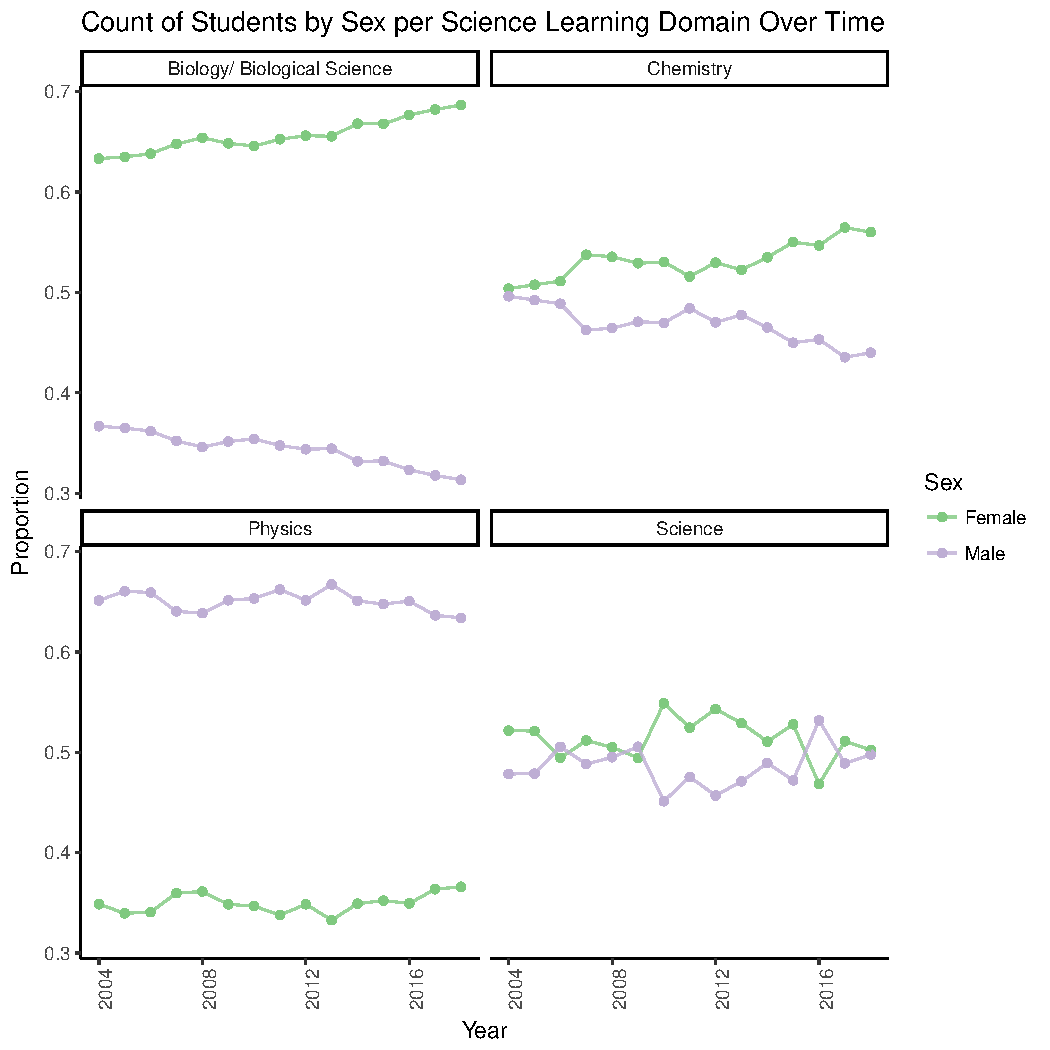
\includegraphics{C2 - Student Pathways/STEM_Participation_Y13_Proportion_Science_Sex.pdf}
    \caption{\textbf{Science Participation Rates across years by sex}. These plots show the representation of male and female students in key science subjects in Year 13 from 2004-2018. Biology, Chemistry show a gender balance favouring female students (e.g., nearly 70\% of biology students in 2018 were female). Physics continues to be male dominated. "Science" represents core science papers, and appears to have a relatively balanced representation of male and female students across years. Data retrieved from \cite{EducationCounts_2018}.}
    \label{fig:STEM_Participation_Sex}
\end{figure}

Data from \cite{EducationCounts_2018} also allows us to see trends in STEM participation by school decile, a proxy measure of SES. In New Zealand, school decile refers to the affluence of the neighborhood in which a school is located. High decile schools are located in more affluent areas, whilst low decile schools are located in less affluent areas. As shown in Figure \ref{fig:STEM_Participation_Decile}, students who take science subjects are most likely to come from higher decile schools. Students who take mathematics with either statistics or calculus are also more likely to come from high decile schools. The relationship between student enrolment in technology learning domains and decile follows no clear pattern.  
\begin{figure}
    \centering
    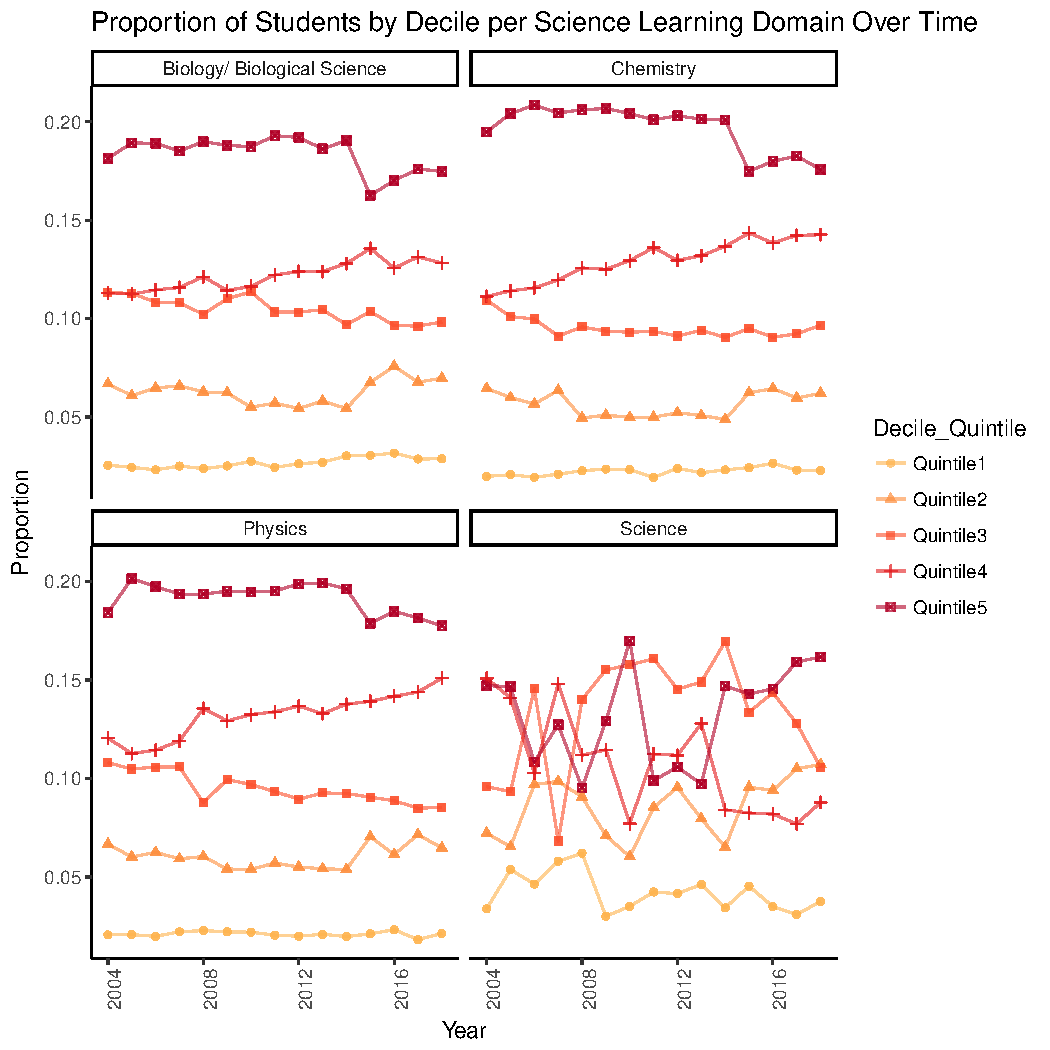
\includegraphics{C2 - Student Pathways/STEM_Participation_Y13_Proportion_Science_DecileQuintile.pdf}
    \caption{\textbf{Science Participation Rates across years by school decile}. School deciles are grouped into quintiles (decile 1 and 2 schools into decile 1, decile 3 and 4 into quintile 2, and so on). As can be seen in the above plots, students were more likely to take biology, chemistry, and physics if they attended high decile schools. The plot of the core "Science" subject appears less ordered, indicating that trends follow a less clear pattern. Data retrieved from \cite{EducationCounts_2018}.}
    \label{fig:STEM_Participation_Decile}
\end{figure}

Whilst broad level data, such as those discussed above, do allow us to interpret trends in subject enrolments over time, they provide only a surface level understanding of STEM participation. Beneath the aggregation of counts per subject label hides important information that are useful for policy makers and researchers. By considering participation at the level of individual standard assessments, we are able to disentangle assessment patterns within subject, and between subject. We can also explore factors related to individual standards, (such as the type of standard assessment and whether it was assessed internally or externally). To build on and inform the broad level understandings outlined previously, we adopt the following research questions:
\begin{itemize}
    \item Can we identify patterns in the NCEA Level 3 standards  taken by students STEM?
    \item If so, how do the patterns of NCEA Level 3 standard enrolments differ across demographic characteristics, SES, and year?
\end{itemize}

Given that NCEA can be considered ``one of the most complicated education system in the world'' \citep{hipkins2016ncea}, unpacking details at a finer grain level can be a daunting task. In order to explore this complicated system and answer our research questions, we employ quantitative techniques based in the field of network analysis. We explain how network analysis may be used as a tool to understand patterns of assessment, especially in contexts where the system is complex (as in NCEA).  This approach may provide a methodology that is useful for education researchers across contexts. 


\subsection{Using Networks to Understand Patterns of Assessment}
A network is a collection of nodes and edges. Nodes can represent an agent (e.g., a student) or an object (e.g., a standard), whilst edges link two nodes together to indicate some form of shared relationship. Networks can be used to represent anything from human relationships, transport networks, biological and computer systems. In education research, network analysis has tended to focus on the relationships shared between students in the classroom \citep{tranmer2014multiple}, or communication between staff at educational institutions \citep{daly2010social}. There are few examples of education research that use network analysis to investigate non-social relationships. We seek to expand this area of research by applying network analysis to high school assessment enrolment data. As outlined in the following section, we use network analysis to understand the patterns of standards that show a preference for being taken together. We then explore how these patterns differ over time, and by gender, ethnicity, and school decile.

The current study will specifically investigate the STEM standards that NCEA Level 3 students enrolled in, and how these community structures relate to student and school level characteristics. Previous research by \citet{ferral2005clustering} employed similar clustering techniques to investigate communities of subjects in NCEA at high school. Ferral's study offers valuable insights into the subjects taken by students, but was limited by the number of schools sampled, the response rate of schools, and the availability of demographic and standard information. The current study is able to address these limitations by accessing administrative data through the IDI for the whole of New Zealand's NCEA Level 3 population between 2010 and 2016. We focus the analysis of the current study to STEM students and their NCEA Level 3 records in order to reduce the scope of our analysis and focus on one specific pathway through education. While the analysis discussed in the current study may be repeated for students engaged in other pathways, we focus on the STEM pathway because it is a stated interest for government. We also focus specifically on students' NCEA Level 3 records, as it is the most highly specialised and precedes entrance to university and the employment market. By NCEA Level 3, students have likely decided on their future career.

\section{Methodology}
\subsection{Data}
We make use of the New Zealand Integrated Data Infrastructure (IDI) to access administrative data pertaining to students' high school and census information. The IDI is a collection of government run data sets, containing data on student enrolment and demographics, tied at an individual level for the whole New Zealand population. We focus on students taking NCEA Level 3 from 2010 to 2016, as this is the most up to date data available at the time of writing. Years prior to 2010 are available, but were omitted due to processing constraints. The years spanning 2010 to 2016 were also of specific interest, due to policy reforms introduced around 2012 and 2013. We apply several rules when selecting student cohorts to minimise the risk of including individuals who do not represent the typical student population and may add statistical noise to the patterns we identify in our network analysis. Firstly, we only select individuals who are identified as having tax, birth or VISA records. We also only include students who had NCEA records when they were 15 or 16 and during NCEA Level 1. These filters help focus our sample on the resident population of New Zealand, and minimise the chances of including visitors or foreign exchange students. We also limit our sample to students who attended state schools in New Zealand. This is because private schools in New Zealand may offer a combination of NCEA and other formal qualifications (such as Cambridge or IB). As students are able to take NCEA Level 3 standards over multiple years, we assign each student a single cohort year based on the most frequent year in which they took standards. For example, if a student took two NCEA Level 3 standards during 2015, and ten NCEA Level 3 standards during 2016, we would assign the student to the 2016 cohort. We choose not to exclude standards taken in a different year from the overall cohort year, as these standards would still contribute to the student's qualification.

We include the following variables in our analysis
\begin{itemize}
    \item Student sex (male or female). Due to limitations in the administrative data used, we are not able to include gender (and non-binary classifications of gender) in our analysis.
    \item Student ethnicity. Each student is able to identify with multiple ethnic groups, following the classification set out by Statistics New Zealand. The main ethnic groups include Pakeha/European, M\={a}ori, Pacific Islands, Asian, Middle Eastern Latin American or African (MELAA), and Other. For the purposes of this study, we do not report results for MELAA and Other.
    \item High school decile. This is a rating out of 10 for the affluence of the area where the school is located. For the purposes of the current study, we categorise high school decile into 3 groups. Deciles 1-3 are low decile, deciles 4-7 are medium decile, and deciles 8-10 are high decile. 
    \item NCEA Level 3 standards taken. For each student, we have information on all of the standards taken at NCEA. We only include standards from the New Zealand Curriculum learning areas of Science, Technology and Mathematics \cite{NZCurriculum2007}. For each standard, we have information on its learning domain (e.g., physics, biology, mathematics etc.), whether it was a unit or achievement standard, and whether it was assessed internally or externally.
\end{itemize}

\subsection{Network Analysis}
We employ network analysis to understand STEM enrolment at NCEA Level 3 at a fine-grained level. Our nodes take the form of students and standards. Edges in our network represent any recorded instance where a student took a standard during secondary school. This represents a bipartite network (also commonly referred to as a two-mode network). A bipartite network is any network where there are two types of node, and nodes can only connect to a node of a different type. In our case, a standard cannot be connected directly to another standard, and a student cannot be connected to another student. For example, in \ref{fig:BipariteNetwork}, standards may be represented by nodes in set A, whilst students may be represented by nodes in set B.
\begin{figure}
    \centering
    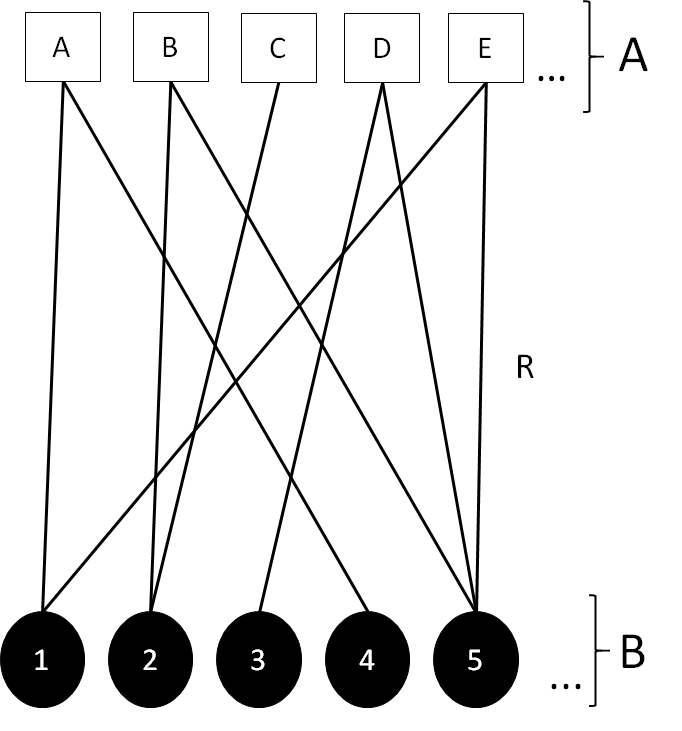
\includegraphics{C2 - Student Pathways/Bipartite_Network.png}
    \caption{\textbf{An Example of a Bipartite Network}. In the case of the current study, white nodes (set A) represent standards, whilst black nodes (set B) represent students. If a student took a particular standard, this is represented by an edge R.}
    \label{fig:BipariteNetwork}
\end{figure}

We generate a network of students and the standards they were enrolled in for the whole of our student population. We structure this network so that it is multidimensional. Each student node belongs to a specific year, region, and decile, while standards can exist across multiple years, regions, and deciles. In order to analyse the properties of our network, we are required to `project' onto one set of nodes. This means that we take one set of nodes type, and generate edges between these nodes when they share an indirect relationship through the other node type. For example, \ref{fig:BipartiteNetwork_Projection} shows the projection of \ref{fig:BipariteNetwork}. In this case, standards represented in set A are now connected to one another, and students in set B are also now connected. 
\begin{figure}
    \centering
    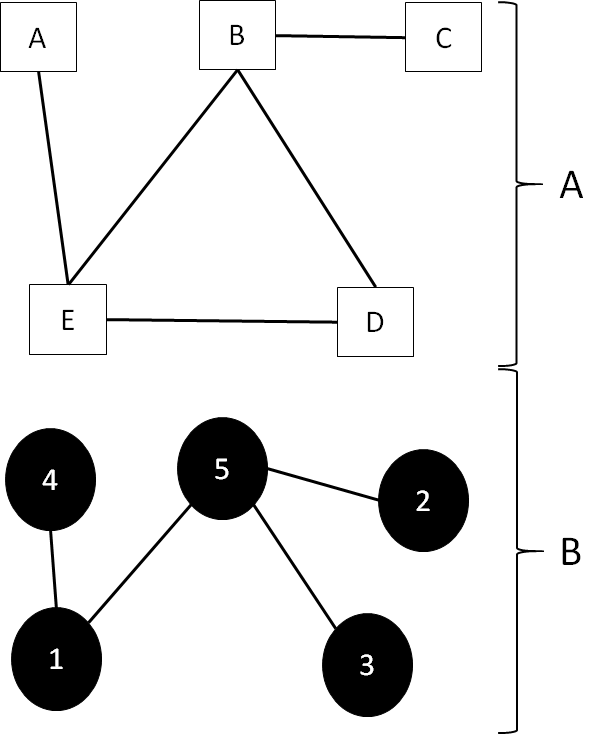
\includegraphics{C2 - Student Pathways/Bipartite_Network_Projection.png}
    \caption{\textbf{An Example of a Bipartite Projection}. Nodes within either type now connect to one another. Edges now indicate that two nodes share an indirect relationship through a node belonging to the other set of nodes.}
    \label{fig:BipartiteNetwork_Projection}
\end{figure}
As we are interested in the patterns of standards that students took, we project onto the standard nodes. This results in a network of standards that are connected by edges indicating that students took those two standards together within their NCEA Level qualification. The edges of the projected standard network can also take on a weighting that corresponds to the frequency that two standards were taken together. This weighting provides the number of students that took those two standards together. The multidimensional nature of the original network means that there are several different type of edge in the projected network (in network science, this is refered to as a multiplex network). 

\subsection{Normalization and Community Detection}
Our goal is to use the networks to understand the standards that tend to be taken together, and by which students. To do this, we employ community detection. Community detection is a process in which we identify nodes that are `grouped' together due to the edges in the network. Usually community detection methods identify communities by maximising the \textit{modularity} score within communities. Modularity refers to the tendency of nodes to connect to other nodes within the same community more than nodes that are outside of the community. Whilst there are many different community detection algorithms, the current study makes use of the Map Equation \citep{rosvall2009map}. 

In order for our communities to truly represent the standards that tend to be taken together, we need to normalize our edges so that weights do not refer to the raw frequencies of students between standards. The raw weighting does not consider the fact that standards have different populations of students. As a result, community detection may group two standards together simply because one standard has a large number of students. To explain more clearly, we can use the hypothetical case of English Standard A, Physics Standard A and Physics Standard B. If English Standard A has a population of 1000 students, and 10\% of those students take Physics Standard B, the raw weight is 100 students. If 100 students took Physics Standard A, and 90\% of those students took Physics Standard B, the raw weight is 90 students. This shows how using the raw number of students as edge weights may not give us the communities of interest. Instead, we make use of a normalization technique called Revealed Comparative Preference (RCP). RCP measures the fraction of students from standard $j$ who also took a second standard $i$, relative to the overall fraction of students taking standard $i$, across all other standards. More specifically: 
$$RCP(i,j) = \frac{x_{ij}/x_j}{x_i/x}$$
where $x_{i,j}$ is the number of students taking both standard $i$ and $j$, $x_j$ ( or $x_i$) is the total number of students taking standard $j$ (respectively, course $i$), and $x$ is the total number of unique students enrolled in any standard. This RCP metric is based on the measure Revealed Comparative Advantage, used in economics \citep{Balassa1965}, and was calculated using the EconGeog package \citep{balland2017economic}. The RCP calculation returns a value where anything greater than 1 indicates a preference for two standards being taken together. A value below 1 indicates that, given the number of students in either standard, there was no preference in the two standards being taken together. 

We remove any edge in the network where the RCP value is below 1, and subsequently any node that no longer has any edges (nodes with a degree of 0). Our network now consists of standards connected by edges with a weighting relative to the preference for each standard being taken together in NCEA Level 3. The next step is to identify communities of standards that are grouped together in our network. To identify communities, we use the infomap community detection method \citep{rosvall2009map}. In basic terms, the infomap community detection algorithm partitions the network in a way that maximizes the number of edges within a community, compared to the outgoing edges between communities. 

\subsection{Exploring Participation}
To compare student participation across the educational fields detected, we can consider the relative proportion of students from particular years, and across school deciles and social groups. One of our goals is to establish an overall idea of how each network is structured. Are the enrollments for a specified group spread more evenly across a network, or are they focused in particular areas? To answer this question, we employ a measure of entropy. Entropy is a concept adapted from thermodynamics which provides an indication of how organised or disorganised a system is. In the case of the current study, we use entropy to assess how participation is spread across the network. Using the measures of entropy as signals of disparities, we then explore the rates of participation across communities and standards in finer grained detail. The following sections will outline our measure of entropy, and our how we then explore trends in the structure of the network in more detail. 

\subsubsection{Entropy}
To explore how the structure of our network of assessments differs across social groups, we employ a measure of \textit{entropy}. Entropy provides an aggregated metric of how ordered a system. Systems that are highly ordered have a lower level of entropy, while disordered systems have higher entropy. To use an analogy, solid objects have low entropy, while liquids have higher entropy. Following this analogy, we may explain high levels of entropy in our network of assessments as indicating that a sub-population's patterns of enrollment is more widely spread across the network (more fluid). Lower levels of entropy indicate that a sub-population's pattern of standard enrollments is more focused or specialised. By partitioning our network into different social groups (e.g., across gender, ethnicity and school decile) we can explore similarities and differences in network structures. 

We calculate entropy in two steps. Firstly we work out the probability of a sub-population enrolling in a specific standard given the total number of enrollments for that sub-population. This probability is given by:
$$p_i = \frac{q_i}{T}$$
where $q~_i$ is the number of students in a sub-population enrolled in standard~$~i$, and $T$ is the total number of enrollments for that sub-population. Using this measure of probability, we calculate entropy using the following formula: 
$$S = -\sum_{i}^{N}{
\frac{p_i\log{p_i}}{\log{T}}
}$$


Where $p_i$ is the probability of a student from the population considered enrolling in standard~$_i$ given the overall total number of enrollments for that population ($T$). Alternative normalisation are possible. For example we could normalise by the number of standards in the network. This would be equivalent to assuming that the probability of a student enrolling in a specific standard is independent of the standard. This assumption does not hold for two reasons. Firstly, standards have very different numbers of student enrollments. Secondly, different student groups are differently represented in different standards. In contrast, normalising by $T$ accounts for the number of students from a sub-population enrolled in a specific standard. However, it does not let us distinguish between effects due to the size/popularity of a standard and those due to differing preferences of specific populations for specific standards. A downfall of this approach is that it does not account for standards that no enrolments for students in a specific sub-population.

We ascertain a level of confidence by using a bootstrapping method, where we randomly vary the population in each standard by 20\%, and recalculate entropy. We repeat this process 1000 times for each entropy measure. 

\subsubsection{Trends}
Following the entropy measure, we investigate how participation differs across demographic groups per standard by comparing raw counts, proportions, and probabilities. The communities identified provide a good idea of the standards that tend to be taken together, which allows us to explore rates of participation across groups of standards as well as individual standards. We are able to explore a range of attributes, such as such as the probabilities of sub-populations enrolling in a standard, with respect to gender, ethnicity, school decile, and type of standard (achievement/unit standards, internally/eternally assessed).  

Following the detection of different communities of standards, our goal is to explore the student enrolment patterns in these communities. Based on trends outlined by \citet{EducationCounts_2018}, we make the following hypotheses:
\begin{itemize}
    \item Female students will be more likely to have enrolled in standards in communities related to biology.
    \item Male students will be more likely to have enrolled in standards in communities related to physics, calculus and computer science.
    \item Students who attended high decile schools will be more likely to have enrolled in externally assessed standards.
\end{itemize}
Less research has investigated the relationship between assessment type (achievement or unit) and STEM enrolment, but we may expect that students groups who historically succeed in traditional forms of education (high SES, European and Asian students) to be more likely to have enrolled in externally assessed achievement standards. Student groups who have historically been under-served by traditional assessment may be more likely to have enrolled in unit standards. 




\section{Results and Discussion}
\subsection{Exploring Participation}
To investigate our hypotheses, we first generated a complete network of all students across all years, regions, and deciles (Figure \ref{fig:NetworkAll}).

\begin{landscape}
\begin{figure}
    \centering
    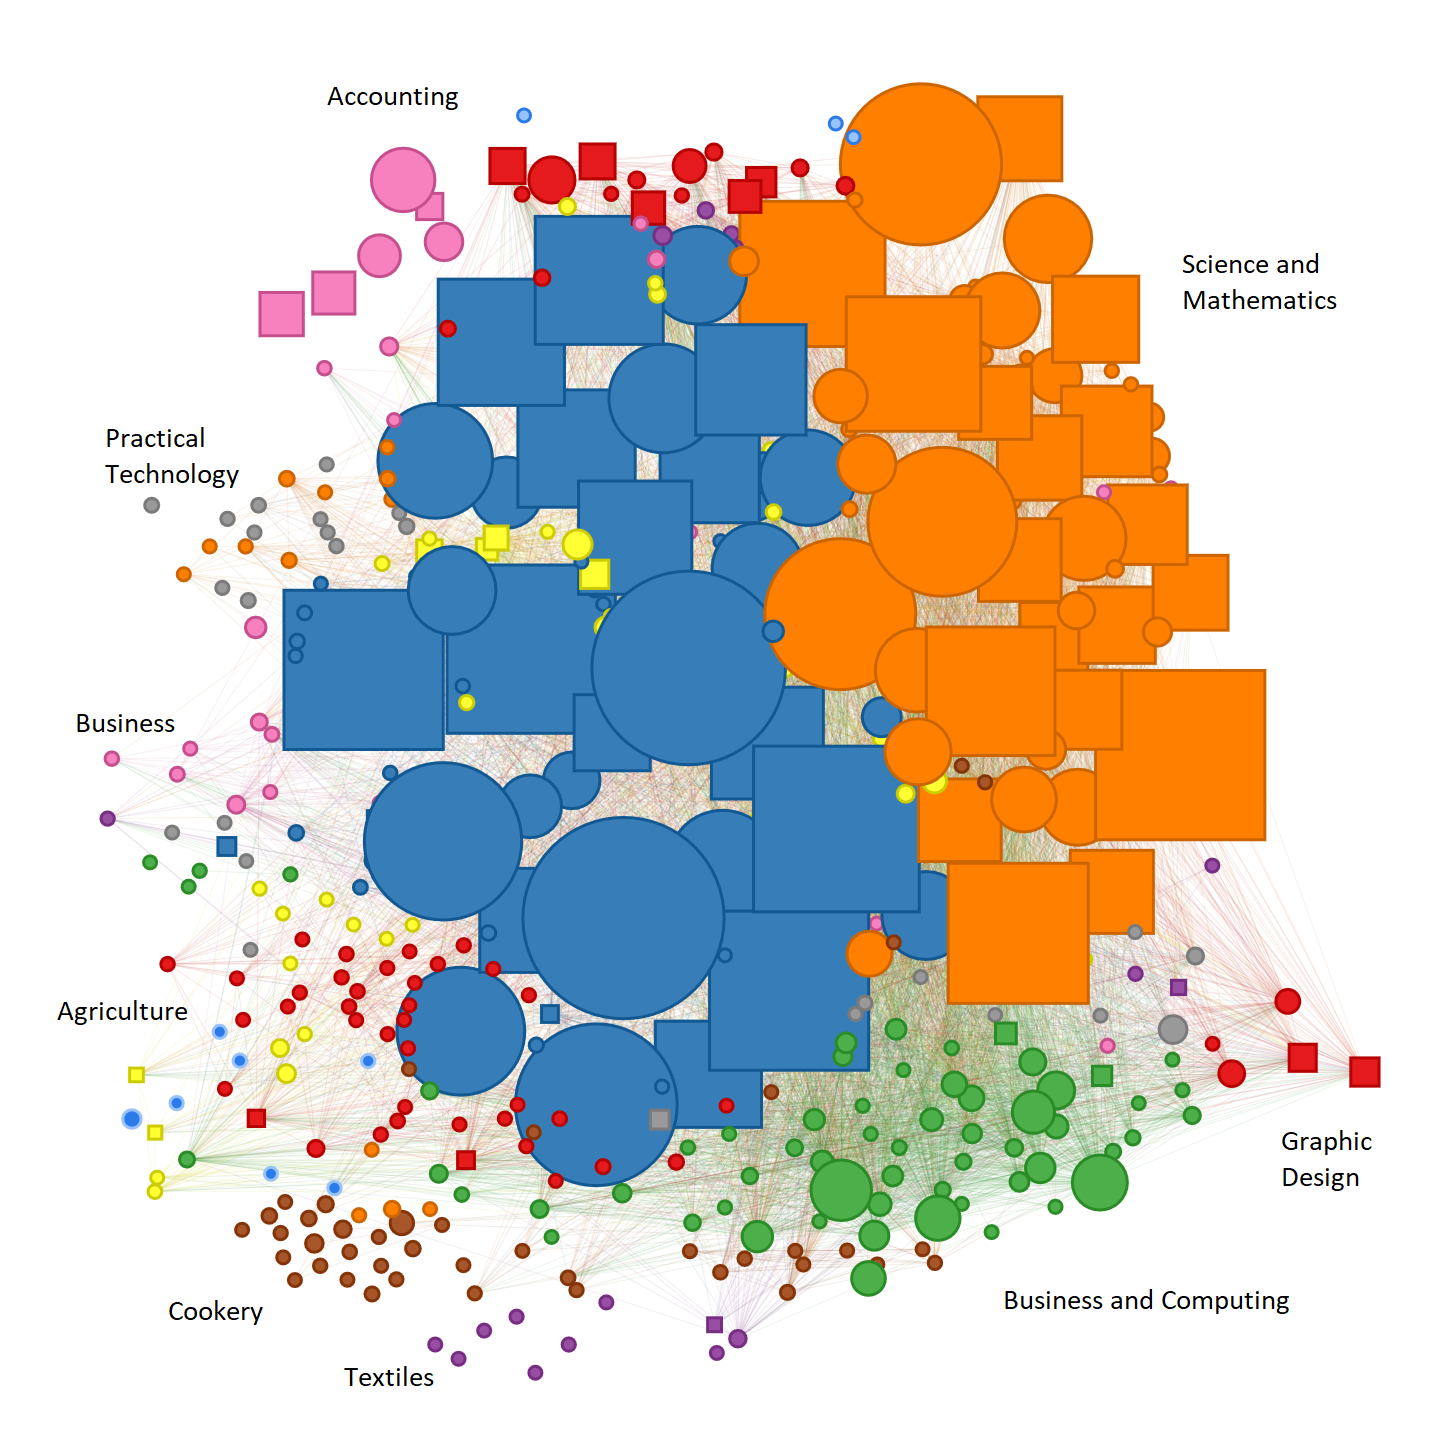
\includegraphics[width = \textwidth]{C2 - Student Pathways/L3NCEA_STEM_Network_All.png}
    \caption{\textbf{Network of NCEA Level 3 standards}. The standard projection of the NCEA Level 3 student-standard network. Nodes represent standards that students may enrol in, whilst edges represent a preference for two standards being enrolled in together. Colours represent the communities of standards that tend to be taken together. The above network includes all standards offered between 2010 and 2016.}
    \label{fig:NetworkAll}
\end{figure}
\end{landscape} We normalised the network using RCP and then detected community structures in the network using the Map Equation \cite{rosvall2009map}. We found that the communities of assessment revealed differed in size and composition across each year, region, and decile. This is an expected finding, given that different schools may offer different standards, and that standards are introduced and removed from operation over years.

The Map Equation community detection algorithm identified 42 communities of Level 3 STEM standards. As NCEA Level 3 is the most specialised stage of high school education, we would expect our network to be strongly partitioned into different community structures. This is reflected in a high modularity score of 0.83. The modularity score indicates that the detected communities tended to have more edges between nodes within communities than between communities. 

The structure of the network did change over time, with a significant change taking place between 2012 and 2013. During this time, a change in policy resulted in a reform in assessment. Science and mathematics linked unit standards were phased out, and a new set of achievement standards were introduced. Post this 2013 reform, the overall number of standards diminished, and the network is mainly dominated by one community of mathematics and science standards (see Figure \ref{fig:NetworkYear}). This policy change is also reflected in changing levels of entropy in the network over time. As shown in Figure , the overall entropy of the network of assessments (taking all students into account) decreased over time. This may be an indication that, following the reforms to standards in 2013, student enrolments were more standardised and focused, and less flexible and spread.


\begin{landscape}
\begin{figure}[h]
    \centering
    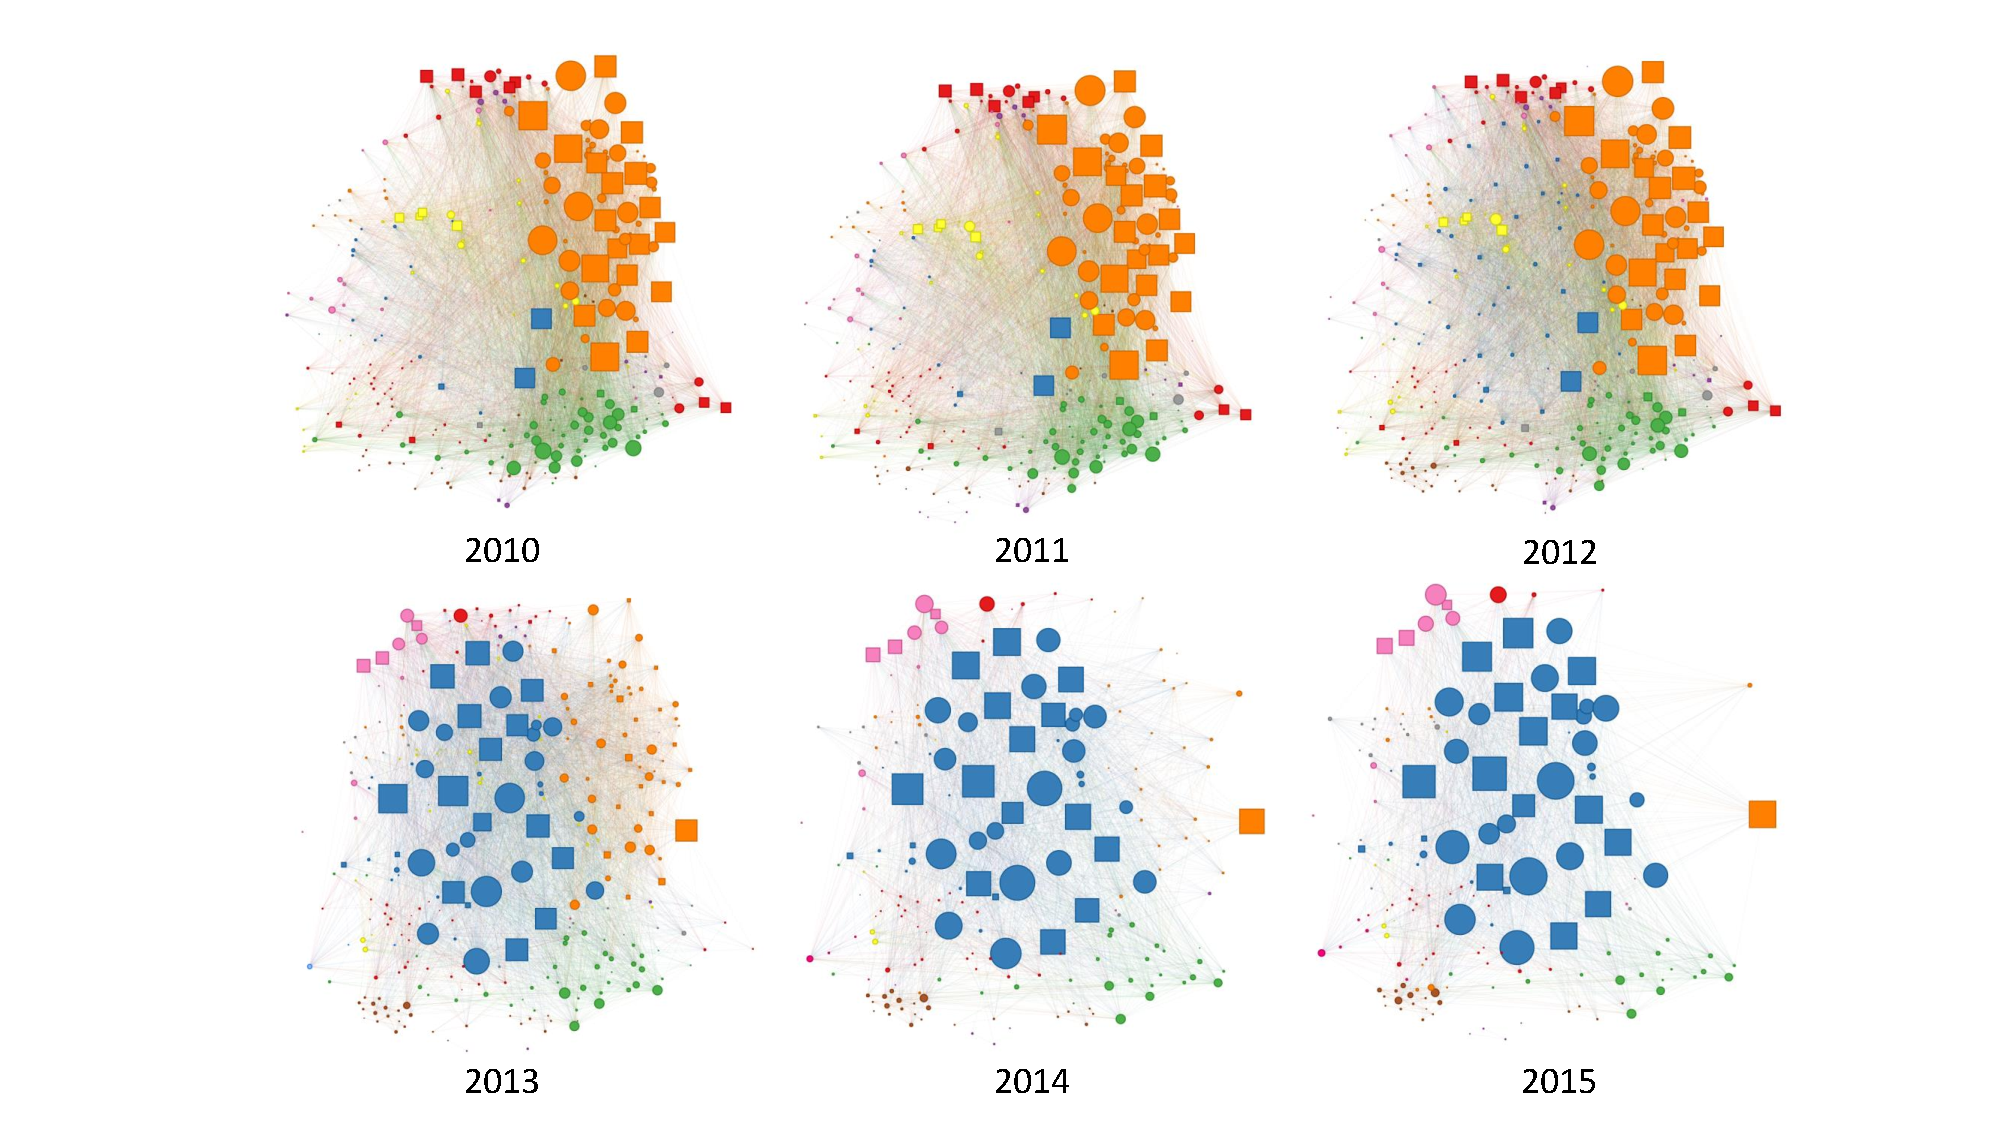
\includegraphics[width = \textwidth]{C2 - Student Pathways/NCEA_Level3_network_year.pdf}
    \caption{\textbf{Network of NCEA Level 3 standards across years Year}. The standard projection of the NCEA Level 3 student-standard network by years. Nodes size represents the relative proportion of students enrolled in each standard. As years progressed, the number of standards was reduced. Around 2013, a new set of science and mathematics achievement standards were introduced. Post 2013, the network is comprised mainly of one mathematics and science community, which indicates that assessment was more standardised than previous years.
    }
    
    \label{fig:NetworkYear}
\end{figure}
\end{landscape}

Through the use of network analysis we are able to summarise and explore a wealth of data, and delineate the main fields of study that comprise NCEA Level 3 STEM. Our method of using RCP and community detection separates out standards according to their propensity for being taken together, and not by their subject label. The detected communities may thus provide a clearer picture of NCEA enrolment than broader subject labels. To provide an example, the chemistry standard \textit{Evaluate the interaction of a chemical process with society and/or the environment} may not assess the same content knowledge as another chemistry standard \textit{Demonstrate understanding of the properties of organic compounds}. Despite both standards belonging to the domain chemistry, they were placed in separate communities in our network. Nevertheless, on the whole, the communities in the network tended to be comprised of standards from the same domain of study. For example, biology standards tended to be taken in conjunction with other biology standards. Whilst this is unsurprising, we also find that communities tend to be comprised of standards from multiple domains. For example, the largest science-related community consists of standards from mathematics, biology, physics and chemistry. We argue that the combination of RCP and community detection provides an unbiased method of revealing the specialized fields of STEM education that go beyond subject label. We now detail some trends that can be observed from 2010 to 2016 by gender, ethnicity and school decile, discussing how this contributes new insights beyond the discussion of broad level patterns outlined previously.

The following section outlines some of the key findings by gender, ethnicity, and school decile. While there are a vast number of interesting trends to be explored, we focus our discussion on a few key examples. Through these examples we seek to highlight the additional insights that can be gained through investigating NCEA at a fine grained level. We discuss these examples in the context of prior research and the broader patterns of enrollment outlined previously. We provide the reader with the opportunity to explore the network if they are seeking answers to more specific questions (\url{https://stur600.shinyapps.io/Explore_NCEA_L3_STEM/}). 

\subsection*{Summary of participation by gender, ethnicity and school decile}

\subsubsection*{Gender}
Overall, there were small differences in the levels of entropy in the network by gender, with male students tended to have higher levels (see Figure \ref{fig:Entropy_Gender}). This finding would suggest that the male sub-population of the network had more similar probabilities of enrollments spread across the network, while the probabilities of enrollments for the female sub-population were more focused in specific areas. Further investigation of communities in the network showed clear examples of gendered subject disciplines which may explain the difference in entropy. Male students tended to dominate communities defined by standards in the agriculture, engineering, and practical technology (welding, furniture making etc.) domains, while female students had greater rates of enrolments in standards related to life sciences and textiles. 

\begin{figure}[h]
    \centering
    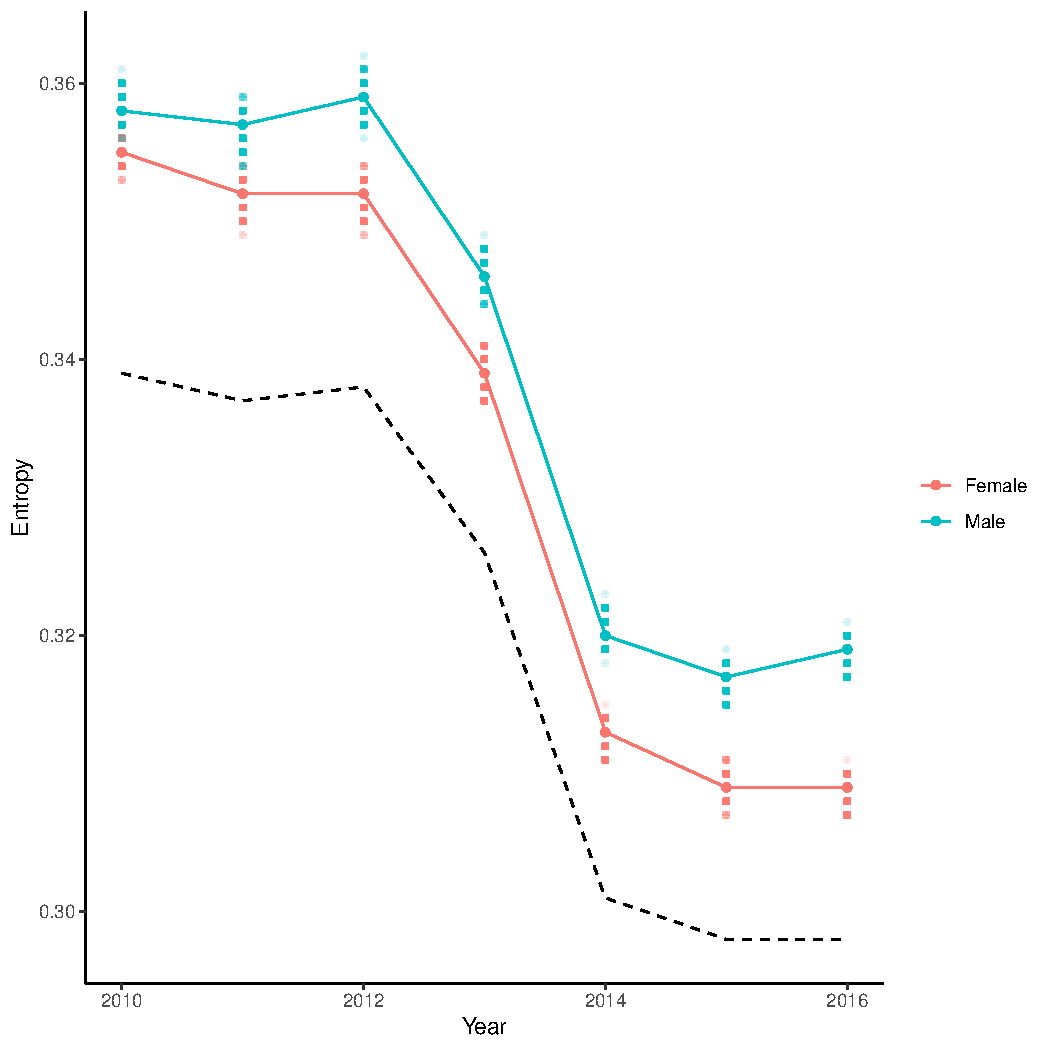
\includegraphics[width = \textwidth]{C2 - Student Pathways/Entropy_Gender.pdf}
    \caption{\textbf{Entropy by gender across years}. Results show that entropy tended to be higher for the male sub-population (blue) than the female sub-population (red) and the population taken as a whole (dotted black).
    }
    
    \label{fig:Entropy_Gender}
\end{figure}


The main science communities also tended to be slightly male dominated (53\% for the main science community prior to 2013 reforms, and 51\% for the main science community post the reforms in 2013). With that being said further exploration of the main science communities reveals more specific gender differences in subject domains. Female students tended to be more likely to be enrolled in standards relating to biology, with the majority of biology standards having around 60-70\% female students across academic years. Female students were also more likely to have enrolled in standards in the Core Science domain, which includes standards such as \textit{Research a current scientific controversy} (61.5\% female) and \textit{Describe genetic processes} (67.3\% female). Female students were less likely to be represented in calculus and physics standards than male students (see Table \ref{table:StdattainmentGender}). 

\begin{table}[ht!]
\begin{tabular}{|c|c|c|c|}
\hline
Standard & Assessment Type & Domain   & Female (\%) \\ \hline
     Differentiate functions and use derivatives to solve problems & EX & Calculus & 38.2\\
      & & & \\
     Integrate functions and use integrals to solve problems & EX & Calculus & 38.3\\
      & & & \\
     Differentiate functions and use differentiation to solve problems & IN (Unit) & Calculus  &    42.3   \\
     & & & \\
     Integrate functions and use integration to solve problems & IN (Unit) & Calculus & 46.3\\
      & & & \\
      Demonstrate understanding of wave systems & EX & Physics  &  35.2\\
      & & & \\
     Demonstrate understanding of electrical systems & EX & Physics  & 34.7 \\
      & & & \\
      Demonstrate understanding of mechanical systems & EX & Physics & 36.2 
      \\ \hline
\end{tabular}  \caption{The percentages of female students enrolled in specific calculus and physics standards in the main science communities show that female students tend to be underrepresented in calculus and physics standards.}  \label{table:StdattainmentGender}

\end{table}

The rates of enrolment for female students in the physics standards were low, with the proportion of female students in externally assessed physics standards being around 35\% overall. The participation of female students in the standards related to calculus were also low compared to male students, with the proportion of female students being around 35-38\% in the main externally assessed standards. The internally assessed unit standard equivalents of the calculus standards, which were available to students prior to 2013, had an increased proportion of female students (around 42-46\%). 

The rates of participation across the network of standards reflects the broad patterns of participation discussed previously using in subject enrollment data from \citet{EducationCounts_2018}. These patterns also reflect those across international contexts \citep{Else_Quest_2013, Sheldrake_2015, NSF, InstituteofPhysics_2013}. The trends show that in science, female students were more likely to enrol in biology, and less likely to enrol in physics and calculus. Much research has been dedicated to understanding why these trends persist \citep{Blickenstaff_2005,cheryan2017some}, with research often suggesting that female students tend to be less confident in mathematics and calculus compared to male students \citep{Hofer_2016, Heilbronner_2012, Simon_2015}. Whilst differences in confidence may explain why students are less likely to pursue a subject, it does not inform us on the source of disparities. \citet{cheryan2017some} offer a detailed review of why some STEM domains are more balanced than others. 


\subsubsection*{Ethnicity}
Overall, the M\={a}ori and Pacific groups tended to have higher levels of entropy, while Asian and European students had lower levels (see Figure \ref{fig:Entropy_Ethnicity}). The increased spread for the M\={a}ori and Pacific sub-populations is likely related to fewer enrollments in science and mathematics, and relatively more enrollments in vocationally orientated standards. This means that the probabilities of enrollments are spread across the network, while Asian and European students tend to have enrollments focused in science and mathematics.  Secondly, M\={a}ori and Pacific students may be more likely to be enrolled in contextually-relevant internal standards, which appear in greater number in the network than the standardised, externally assessed standards --- hence enrollments appear more spread.


\begin{figure}[h]
    \centering
    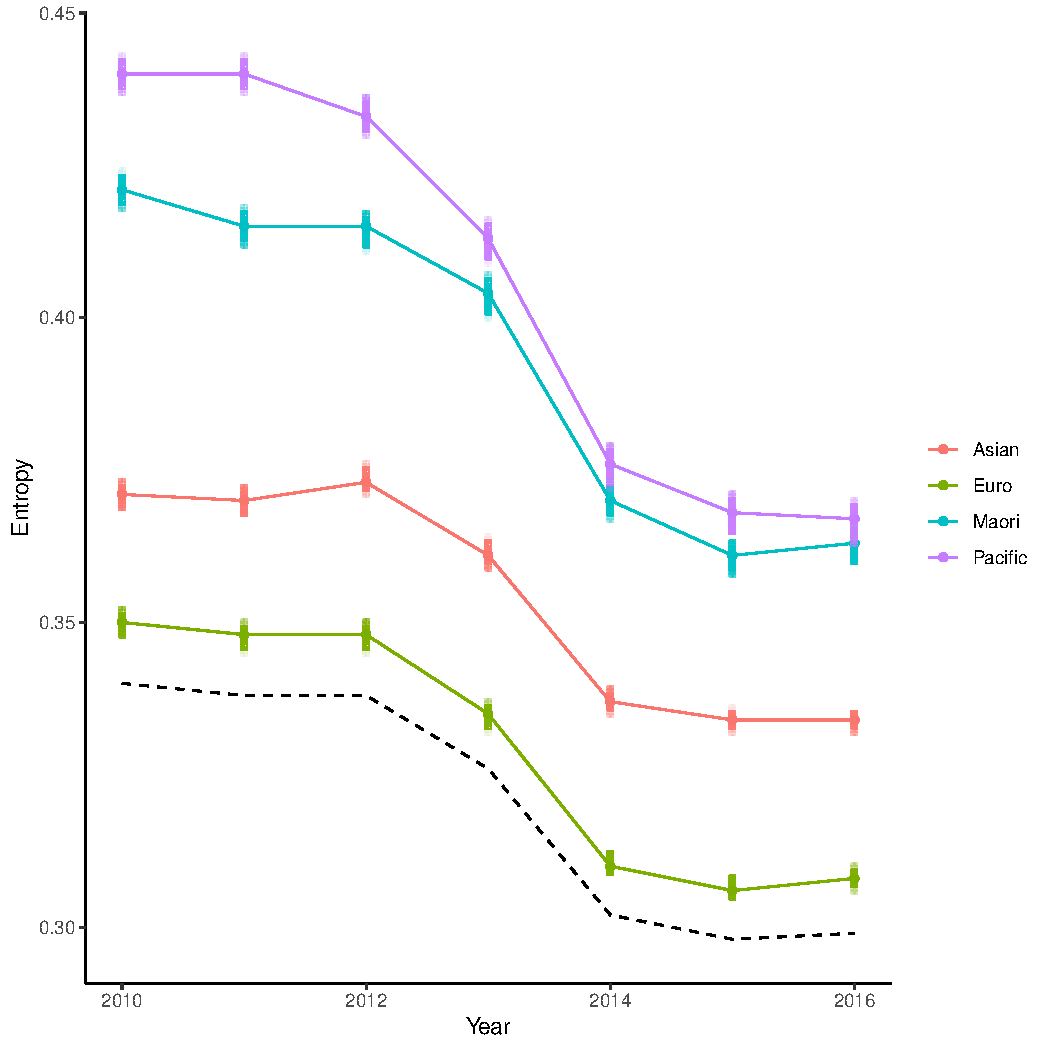
\includegraphics[width = \textwidth]{C2 - Student Pathways/Entropy_Ethnicity.pdf}
    \caption{\textbf{Entropy by ethnic group across years}. Results show that while all sub-populations have higher entropy than the population taken as a whole (dotted black), the M\={a}ori and Pacific Islands sub-populations tended to have the highest levels of entropy. The European sub-population tended to have the lowest levels of entropy. 
    }
    
    \label{fig:Entropy_Ethnicity}
\end{figure}



As can be seen in Figure \ref{fig:NetworkEthnicity}, enrolments for the Pakeha and Asian sub-populations were focused in science and mathematics communities, but the Asian population had slightly higher levels of entropy across years. This trend may be explained in several ways. Firstly, the Asian sub-population appears to have had higher chances of enrolling in accounting standards, as well as mathematics and science standards. Secondly, it is possible that the higher level of entropy can be explained by the spread of enrolments within mathematics and science --- the Asian sub-population had relatively higher chances of taking all mathematics and science standards, while the Pakeha sub-population had a narrow range of standards. Finally, the categorical grouping of ``Asian'' contains an extremely diverse population of students, ranging from India to China, and also including some Pacific Island Nations (e.g., Fijian Indians). The diversity of the population may have been reflected in a diversity of enrollment patterns. 

%\begin{landscape}
\begin{figure}
    \centering
    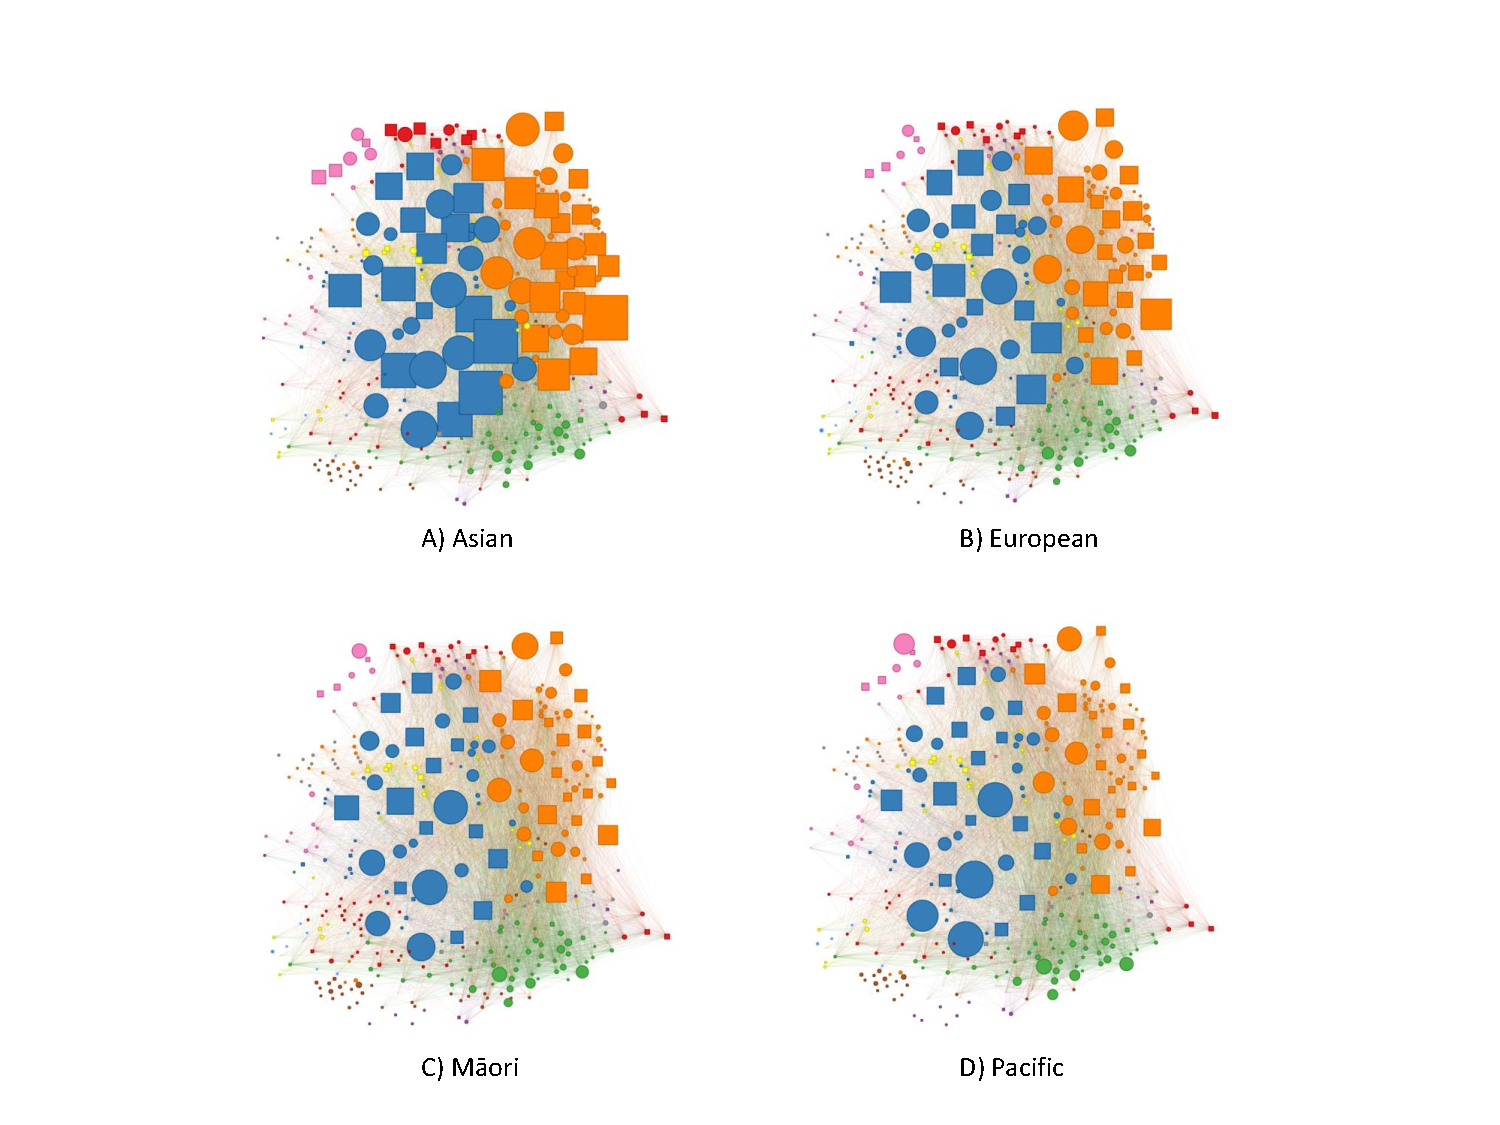
\includegraphics[width = \textwidth]{C2 - Student Pathways/NCEA_Level3_network_ethnicity.pdf}
    \caption{\textbf{Network of NCEA Level 3 standards by ethnic group}. The standard projection of the NCEA Level 3 student-standard network by ethnicity across all years. Nodes size represents the probability of a student from a sub-population being enrolled in a standard. For all ethnic groups, the main science and mathematics communities (orange and blue nodes) tended to have higher probabilities of enrollment. The propensity for science and mathematics standards was especially true for Asian students, and less true M\={a}ori (C) and Pacific Islands (D) groups.
    }
    
    \label{fig:NetworkEthnicity}
\end{figure}
%\end{landscape}

The M\={a}ori and Pacific Islands sub-populations tended to have higher chances of enrollments in internally assessed unit standards offered prior to 2013. As the number of standards diminished over the years from 2010 to 2016, the likelihood of M\={a}ori and Pacific students being enrolled in internally assessed achievement standards in biology did tend to increase. For example, students who identified as M\={a}ori were around 1.63 times less likely to have enrolled in \textit{Research a contemporary biological issue} in 2010. In 2016, M\={a}ori students were around 1.1 times less likely than non-M\={a}ori students to have enrolled in the standard \textit{Carry out a practical investigation in a biological context, with guidance}. Whilst these two standards are not assessing the same topic area, the overall representation of M\={a}ori students in the internally assessed achievement standards did increase over time, ranging from 10-15\% of students in 2010, to around 16-25\% in 2016. A similar trend can be observed for pacific islands students, but not for Pakeha/European or Asian students. The reduced enrolment of the M\={a}ori and Pacific Islands sub-populations in internally assessed unit standards over time, in addition to the uptake in enrolments in science achievement standards, may explain why their is a slightly steeper decrease in entropy over time for these groups compared to the Asian and Pakeha sub-populations (see Figure \ref{fig:Entropy_Ethnicity}). 

The relative proportions of M\={a}ori and Pacific students in physics and calculus has remained consistent over time. For example, of the M\={a}ori students across all regions and deciles in 2010, 12.5\% took the calculus standard \textit{Differentiate functions and use derivatives to solve problems}, compared to 12.8\% of Pacific Islands students, 20.5\% of Pakeha/European students, and 47.1\% of Asian students. For the post-2013 reform equivalent of this standard, \textit{Apply differentiation methods in solving problems}, in 2016 12.7\% of M\={a}ori students took the standard, compared to 15\% of Pacific Islands students, 24\% of Pakeha/European students, and 49.2\% of Asian students. In order to explore these patterns in more detail, we detail trends at the intersection of school decile. 

There are several potential explanations for the ethnic disparities in the types of assessment that students enrolled in. Research suggests that high school teachers tend to have lower expectations for M\={a}ori and Pacific high school students compared to Pakeha and Asian students \citep{turner2015teacher}, and this may be a factor that influences the standards that teachers assign to students. As outlined by one student in a study conducted by \citet{graham2010Maori}:
\blockquote{The teachers decide where the class is at in terms of choosing which standards [Unit versus Achievement]. It's a disadvantage on you because
it depends on what the teacher thinks you can do and what the kids in your class can do.}.  It is also true that external assessment represents traditional forms of high stakes assessment that may not be assess M\={a}ori and Pacific students in a culturally responsive way. NCEA has been positively perceived by M\={a}ori and Pacific parents because it reduces the focus on competition between students, reflecting the key M\={a}ori and Pacific cultural values of collective good \citep{graham2010Maori}.


\subsubsection*{School Decile}

Overall, the level of entropy in the network tends to decrease as school decile increases (see Figure \ref{fig:Entropy_Decile}. This suggests that enrollments in higher decile schools are more standardised and more focused. This is reflected in the rates of participation in the standardised, externally assessed standards, which tends to increase with school decile consistently across years. For lower decile schools, it may be that more students are enrolled in internally assessed standards, which may differ from school to school. The higher levels of entropy for low decile schools may be a consequence of offering more contextualised assessments to students. Previous research has commented on this trend \citep{hipkins2016ncea}. \citet{wilson2017subject} observed that lower decile schools were less likely to have students enrolled in Subject Literacy Achievement Standards, which are achievement standards that can be used as indicators of subject-specific literacy.  

\begin{figure}[h]
    \centering
    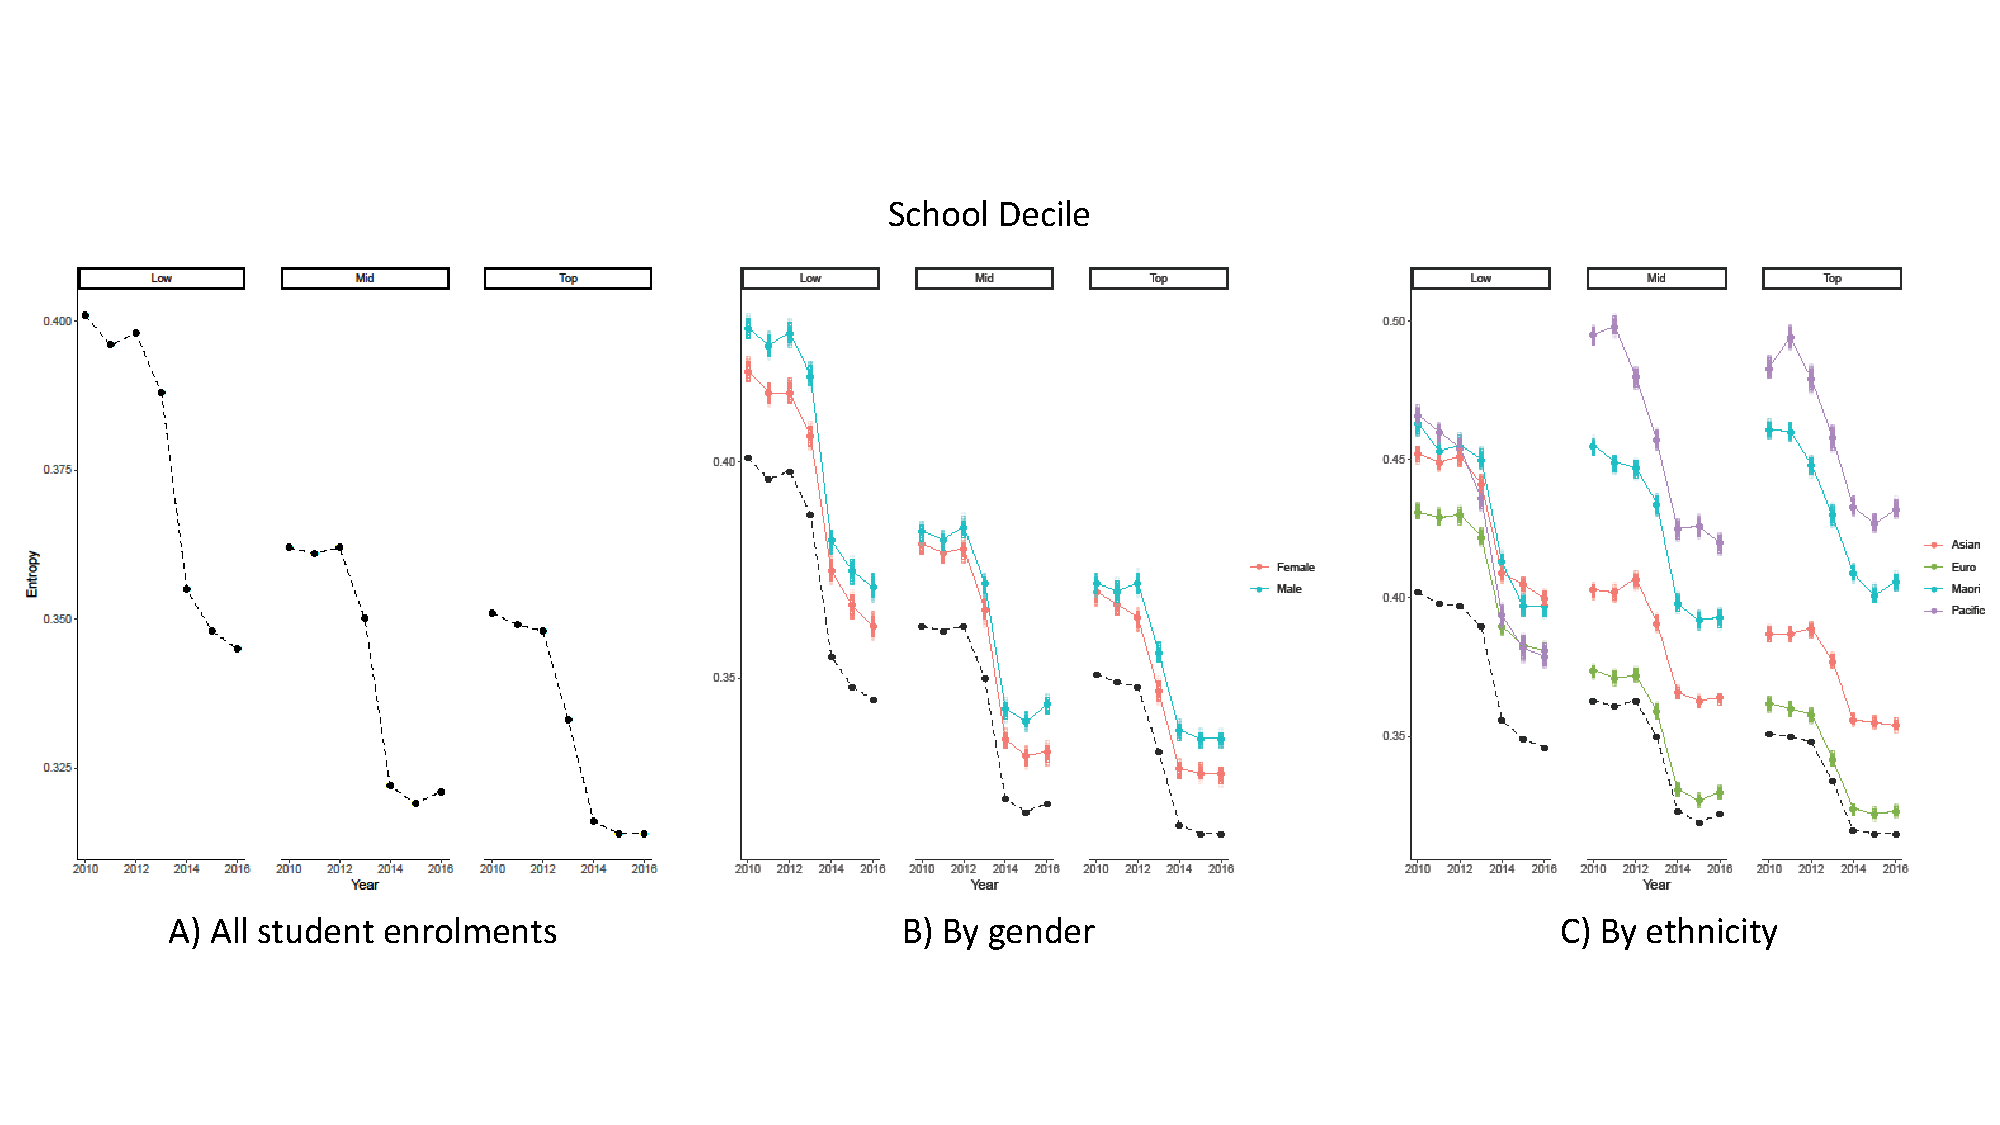
\includegraphics[width = \textwidth]{C2 - Student Pathways/Entropy_Decile.pdf}
    \caption{\textbf{Entropy by school decile across years}. A) The entropy of the network across school deciles for the whole student population. B) The entropy of the network across school deciles split into gender sub-populations. C) The entropy of the network by school deciles split into ethnic group sub-populations. 
    }
    
    \label{fig:Entropy_Decile}
\end{figure}


The standards that students took would be highly, and sometimes exclusively, influenced by the school that they attended. Schools and teachers have the final say on which standards are available to students. The fact that we found that individuals from lower decile schools tended to be more represented in communities of unit standards is an expected finding and reflects the broader trends outline previously. Unit standards provide a valuable type of assessment that prepares students for vocational careers, and it may be that a higher proportion of students from less affluent areas seek vocational careers after high school. While this may explain the relative increase in enrolments in unit standards related to vocations, this does not necessarily explain the increase in curriculum-linked unit standards prior to 2013. Disparities may be explained in terms of a self-fulfilling prophecy on the part of schools. For high decile schools, the normal goal is to attend university, so students are expected to build an NCEA qualification that leads to that goal. In lower decile schools, achieving an NCEA qualification may be the normal expectation, so successfully completing standards and accumulating credits is the focus. It is important to note that in cases where important standards (i.e., those prerequisite for further education) were not available, students were able to enrol in distance learning and complete standards by correspondence. Arguments can be made that providing access by correspondence does is not enough to suggest that all students have the same opportunities. 


Exploring patterns of participation at a finer grain level reveals some interesting insights. With increases in school decile, the disparities in entropy also appear to increase. As shown in C in Figure \ref{fig:Entropy_Decile}, While each ethnic group sub-population tends to have a similar level of entropy in low decile schools, a wider gap is present for middle and higher decile schools. For these schools the level of entropy is lower for Asian and Pakeha sub-populations, and higher for M\={a}ori and Pacific sub-populations. This suggests that the enrolment for M\={a}ori and Pacific students in middle and high deciles schools tends to be more widely spread and less standardised. 

To unpack the disparities in entropy further, we can explore the rates of enrolment for specific standards. We find that ethnic group differences appear to be moderated by decile (see Table \ref{table:StdattainmentEthnicityDecile}). For example, looking at the externally assessed calculus standard \textit{Differentiate functions and use derivatives to solve problems}, we see that in 2010, the standard was taken by around 52.2\% of Asian students from high decile schools, but only 36.2\% of Asian students from low decile schools. For the biology standards related to evolution, a higher percentage of students from high decile schools tended to be enrolled, and this was consistent across ethnic groups and years. Overall, the results provided in Table \ref{table:StdattainmentEthnicityDecile} suggest that school decile does relate to the enrollment choices of students with regards to key science and mathematics standards, and this is particularly true for Asian students. 

In the case of Pacific Islands students studying in STEM in 2010, the percentage difference in students from low and high decile schools enrolled in key science standards tended to be small, with the exception of biology where the disparity by decile was around 10 percentage points (see Table \ref{table:StdattainmentEthnicityDecile}). In 2016, the percentage point differences between deciles tended to be greater, echoing the differences observed for the other ethnic groups. These results suggest that, for Pacific Islands students, the decile of the school had less impact on participation in these standards in 2010 than 2016. 

\begin{landscape}
\begin{table}[h]
\begin{tabular}{lll|l|l|l|l|l|l|l|l|}
\cline{4-11}
          &&& \multicolumn{2}{l|}{\% of Asian} & \multicolumn{2}{l|}{\% of Euro} & \multicolumn{2}{l|}{\% of M\={a}ori}  & \multicolumn{2}{l|}{\% of PI} \\ \hline
\multicolumn{1}{|l|}{Standard} & \multicolumn{1}{l|}{Domain}  & Year & Low & High & Low & High & \multicolumn{1}{l|}{Low} & High & Low & High \\ \hline
\multicolumn{1}{|l|}{Differentiate functions and use derivatives to solve problems} & \multicolumn{1}{l|}{Calculus}  & 2010 & 36.2  & 52.2 & 17.7 & 23.1 & \multicolumn{1}{l|}{11.3} & 15.9 & 13.4 & 15.2 \\
\multicolumn{1}{|l|}{Apply differentiation methods in solving problems} & \multicolumn{1}{l|}{Calculus} & 2016 & 35.4 & 57.3 & 19.0 & 25.7 & \multicolumn{1}{l|}{9.9} & 16.3 & 13.6 & 18.3 \\ \hline
\multicolumn{1}{|l|}{Describe processes and patterns of evolution} & \multicolumn{1}{l|}{Biology} & 2010 & 19.6 & 32.8  & 18.8 & 29.0 & \multicolumn{1}{l|}{10.9} & 23.3 & 7.4 & 17.0 \\
\multicolumn{1}{|l|}{Demonstrate understanding of evolutionary processes leading to speciation} & \multicolumn{1}{l|}{Biology} & 2016 & 27.2 & 33.7 & 24.0 & 31.8 & \multicolumn{1}{l|}{14.6} & 27.3 & 13.6  & 27.6  \\ \hline
\multicolumn{1}{|l|}{Describe aspects of organic chemistry} & \multicolumn{1}{l|}{Chemistry} & 2010 & 25.0 & 40.0 & 14.8 & 24.7 & \multicolumn{1}{l|}{7.4} &16.0 & 10.0 & 12.1 \\
\multicolumn{1}{|l|}{Demonstrate understanding of the properties of organic compounds} & \multicolumn{1}{l|}{Chemistry} & 2016 & 32.0 &42.6 &19.9 &27.9 & \multicolumn{1}{l|}{13.0} & 19.6 &14.2 & 19.6 \\ \hline
\multicolumn{1}{|l|}{Demonstrate understanding of mechanical systems} & \multicolumn{1}{l|}{Physics} & 2010 & 25.4&38.0 &14.7 &23.9 & \multicolumn{1}{l|}{7.0} &16.7 & 8.4&11.0 \\
\multicolumn{1}{|l|}{Demonstrate understanding of mechanical systems} & \multicolumn{1}{l|}{Physics} & 2016 & 30.3&46.4 & 17.4& 27.3& \multicolumn{1}{l|}{8.5} &15.8 &9.6 &17.0 \\ \hline
\end{tabular}
\caption{The percentages of students enrolled in key externally assessed achievement standards in STEM by ethnic group and school decile (low/high). The percentage indicates the number of students belonging to an ethnic group in a particular year who enrolled in the standard, as a function of the overall number of students belonging to that ethnic group in a particular year who took a STEM standard. For example, of the Asian students attending a low decile school in 2010 who took a STEM standard, 36.2\% took the calculus standard \textit{Differentiate functions and use derivatives to solve problems}.  }  \label{table:StdattainmentEthnicityDecile}
\end{table}
\end{landscape}

As can be seen in Figure \ref{fig:PacificDecileMechanics}, the participation of Pacific Islands students in the externally assessed physics standard \textit{Demonstrate understanding of mechanical systems} has improved over time. In 2010, 8.4\% of Pacific Islands students in STEM at low decile schools were enrolled, compared to 11\% at high decile schools. These trends suggest that the participation of Pacific Islands students in this standard has improved since the post-2013 reforms, and this is especially true for Pacific Island students in high decile schools. For example, in 2016, 9.6\% of Pacific Islands students in STEM at low decile schools had enrolled in \textit{Demonstrate understanding of mechanical systems} (a 1.2\% increase over 2010), compared to 17\% at high decile schools (a 6\% increase over 2010). 

\begin{figure}[h]
    \centering
    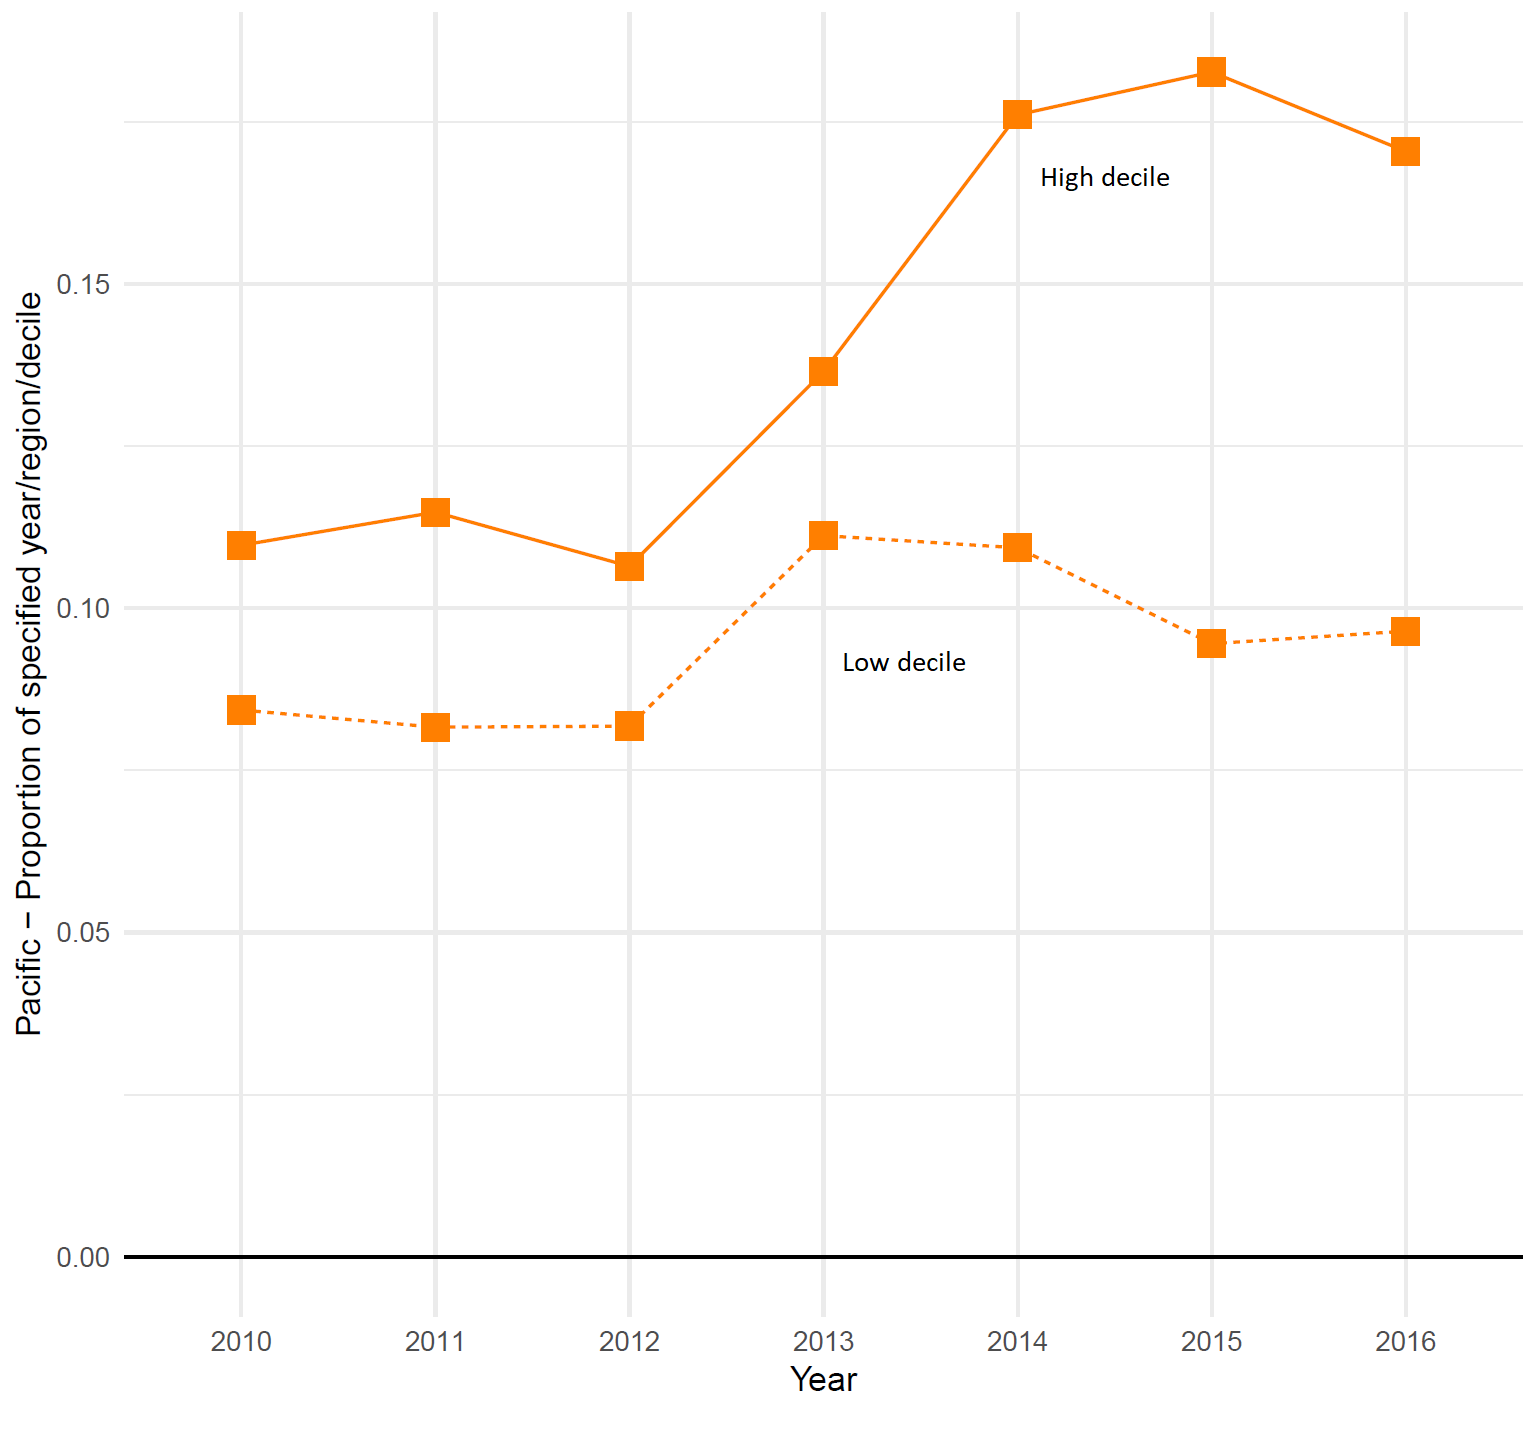
\includegraphics[width=0.9\textwidth]{C2 - Student Pathways/L3NCEA_PacificDecile_Mechanics.png}
    \caption{\textbf{Proportion of Pacific students studying STEM who enrolled in the standard \textit{Demonstrate understanding of mechanical systems} over time and by school decile. }
    }
    
    \label{fig:PacificDecileMechanics}
\end{figure}
The disparities seen in participation in key science standards may be tied to the development of academic identity, and the manner by which it is impacted on by students social location. \citep[p.216]{Archer2014} argue that \blockquote{`cleverness' [can be viewed] as a racialized, gendered, and classed discourse, such that the identity of the `ideal' or `clever' student is not equally open to all students as a viable and authentic identity} This notion of `cleverness' may explain the disparities found in the current study. More specifically, it may be that the 'clever' pathway through NCEA is not open to all students because of factors related to identity (``this pathway is for \textit{me}''). As described by \citet{hipkins2016ncea}, NCEA informally developed into a two-tiered system, with curriculum linked unit standards commonly being viewed an easy pathway, and achievement standards, and especially externally assessed achievement standards, being viewed as a tougher pathway. Students from more working-class backgrounds, or from social groups historically under-served by education, may identify less with the `tougher' academic pathway, even if they had the potential to succeed in it. On the other hand, students with a family background of success in education may be more likely to view the academic pathway as normal or even expected. This idea is described in a related study of high school science pathways in the United Kingdom, where \citet{archer2017stratifying} found that students from more affluent backgrounds were more likely to see the science-orientated pathway as an `obvious' choice. Students from less affluent backgrounds may also be more motivated to seek full time employment, rather than pursue a pathway towards university study and the debt it may entail. However, the question remains as to the extent to which student from less affluent backgrounds knowingly choose vocational pathways and are not channeled down this pathway by simply attended a school in a low SES area -- leading to the second explanation for the disparities observed by school decile.  


\subsection{Implications}
The current study fills a gap in the previous literature by seeking to understand how patterns of standard enrolments at NCEA Level 3 may be related to student gender, ethnicity and social class. We believe that this study is the first of its kind to use bipartite networks to represent high school students' assessment history. Through our methodological approach, we are able to take into account a wealth of information related to students and the standards that they enrolled in. This includes demographic information (gender, ethnicity etc.), and specific NCEA Level 3 standard information, such as the manner in which standards were assessed (externally or internally), and whether the standard was an achievement standard (traditional curriculum based subjects, such as English or science) or a unit standard (more vocational subjects, such as farming or practical technology). Despite growing discussion regarding the outcomes of different types of standards in the New Zealand context \citep{hipkins2016ncea,Lipson2017}, there has been a lack of research into how this information relates to student background. We acknowledge that no single measure of participation is sufficient to fully understand student participation in science \citep{hipkins2005staying}. That being said, we hope that the current study offers a unique perspective that can contribute to our understanding of this area. The methodology described in the following sections allows us to revisit and analyse NCEA as a complex system is rich detail. 


\section{Conclusion}
The current study explored the STEM assessment enrolments of high school students in New Zealand. Through the combination of Revealed Comparative Preference (RCP) and community detection, we were to explore the specific fields of study that students participate in during high school STEM education. Asian students tended to be more likely to be enrolled in science standards characterised by external assessment, whilst students who attended less affluent schools were more likely to take science standards characterised by internal assessment. Female students tended to more likely to be enrolled in science assessments, with the exception of physics and computer science where they were much less likely to be enrolled. We also find that students attending low decile schools, and M\={a}ori and Pacific students, were less likely to be enrolled in the main science community of standards. Whilst it is more difficult to unpack how much of standard enrolment is due to student choice, and how much of it is due to structural inequities present in the school system, our findings reveal inequities in STEM at a fine-grained level. Future research should seek to explore student trajectories through NCEA in more detail.



\section{Disclaimer}
The results in this paper are not official statistics. They have been created for research purposes from the Integrated Data Infrastructure (IDI), managed by Statistics New Zealand. The opinions, findings, recommendations, and conclusions expressed in this paper are those of the author(s), not Statistics NZ. Access to the anonymised data used in this study was provided by Statistics NZ under the security and confidentiality provisions of the Statistics Act 1975. Only people authorised by the Statistics Act 1975 are allowed to see data about a particular person, household, business, or organisation, and the results in this paper have been confidentialised to protect these groups from identification and to keep their data safe. Careful consideration has been given to the privacy, security, and confidentiality issues associated with using administrative and survey data in the IDI. Further detail can be found in the Privacy impact assessment for the Integrated Data Infrastructure available from www.stats.govt.nz. 
